%% Use the hmcposter class with the clinic document-class option.
\documentclass[5pt,clinic]{hmcposter}
\usepackage{tikz}
\usepackage{graphicx}
\usepackage{booktabs}
\usepackage{subfig}
\usepackage{amsmath}
\usepackage{amssymb}
\usepackage{textcomp}
\usepackage{cite}
\usepackage{url}
\usepackage[defaultsans]{droidsans}
\usepackage[T1]{fontenc}


%% For a Clinic poster, there is no author (the author is the team).

%% Project Year.
%% The year is provided using the \year command.
\posteryear{}

%% Project Title.
%% The title of the poster should probably be the name of your
%% Clinic project.
\title{Statistical Interactive Explorer of Vaccine Efficacy}


%% Sponsor's Name.
%% Your sponsoring institution's name.
\sponsor{Nick Kullman, Graham Clenaghan, Wayne Yang - Data Visualization Spring 2015}

%% Sponsor's Logo.
%% The name (base name only; no extension) of an image file with
%% the sponsor's logo.  Ideally, you'll have a PDF version that is
%% resolution-independent.  If not, you'll need a high-resolution
%% PNG file to allow us to print it at a large size without the
%% image becoming blurred.
\sponsorlogo{hmcmath-hexen-logo}

%% Optional -- if your sponsor's logo looks too small or too big,
%% you can adjust its width with the \sponsorlogowidth command.
%% (The height of the logo image is automatically adjusted to
%% preserve the image's aspect ratio.)
%%
%% Note that the argument must be a TeX length; for example, 3in,
%% 5cm, 120pt, etc.  The default width is 2in.
\sponsorlogowidth{0in}


%% Optional -- if your sponsor is hot about their intellectual
%% property and insists on having a copyright statement on the
%% poster, you can use the \copyrightholder command to supply a
%% name for a copyright holder for your poster.
% \copyrightholder{Sponsoring Corporation, Inc.}


%% Define the \BibTeX command, used in our example document.
\providecommand{\bibtex}{{\rmfamily B\kern-.05em%
    \textsc{i\kern-.025em b}\kern-.08em%
    T\kern-.1667em\lower.7ex\hbox{E}\kern-.125emX}}


\pagestyle{fancy}

\begin{document}

\begin{poster}

\section{Problem}
The primary goal of this project is to build a visualization tool to support a technique known as sieve analysis of peptide sequence data from vaccine clinical trials where the vaccine demonstrates partial efficacy.  

\subsection{Sieve Analysis}
Sieve analysis aims to compare the protein sequences of the viral strains which are found in the placebo group against the protein sequences of the viral strains found in the vaccine group using a variety of statistical methods \cite{edlefsen2014comprehensive}.  The vaccine can be thought of as a barrier which filters the viral strains observed in the vaccine group.

\begin{figure}
\includegraphics[height=7in,width=12in]{sieve.png}
\caption{}
\end{figure}

\subsection{Prior Work}
Our project aimed to extend visualizations from the paper \cite{edlefsen2014comprehensive}, in particular figure 2 and figure 3 shown below:

\begin{figure}
\includegraphics[width=12in]{fig2-cropped.png}
\caption{from \cite{edlefsen2014comprehensive}}
\end{figure}
\begin{figure}
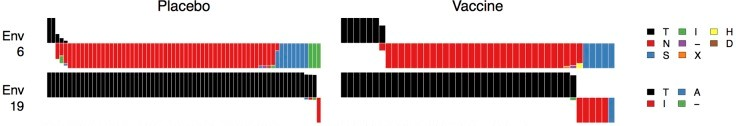
\includegraphics[width=12in]{fig3.jpg}
\caption{from \cite{edlefsen2014comprehensive}}
\end{figure}

Figure 2 shows an overview of the genome for the Env protein with specific sites annotated, and figure 3 shows the distribution of mismatches at two specific sites. The figures were generated with a python script which was run after a statistical analysis determined the sites of interest. We hoped to speed the analysis process through interactivity and then once sites of interest are found, generate usable graphics automatically.

\section{Motivation}
AIDS and other viral diseases such as influenza and dengue claim hundreds of thousands of lives each year.
To assess the efficacy of vaccines built to combat these diseases, researchers apply statistical methods to the results of clinical trial. Sieve analysis is one such method.

Sieve analysis requires determining which sites in the peptide sequence show statistically significant differences in amino acid expression (mutations) between vaccine and placebo groups.
Finding these sites is a labor-intensive process.
The effort involved in scanning for important sites in the sequence increases the likelihood of overlooking them.
A better tool is needed to increase the speed and ease of browsing peptide sequences and the vaccine- vs. placebo-group differences that exist at each site.
Providing this tool will improve the assessment of vaccine efficacy, resulting in quicker turnaround times between vaccine deployments, more effective vaccines, and fewer lives lost.



\section{Approach}

Our goals in designing the interface were the following:
\begin{itemize}
\item Sequence viewing software should be somewhat familiar to researchers.
\item Sites of potential interest should be quickly identifiable.
\item Sites of known interest should be easily found.
\end{itemize}

To accomplish this, we decided to break the tool into three parts: an overview showing a summary of the entire data and the ability to drill down and select particular parts, and then once a selection is made, both a summary of the overall statistics and relevant charts for each selected site.

\subsubsection{Selection}
\begin{center}
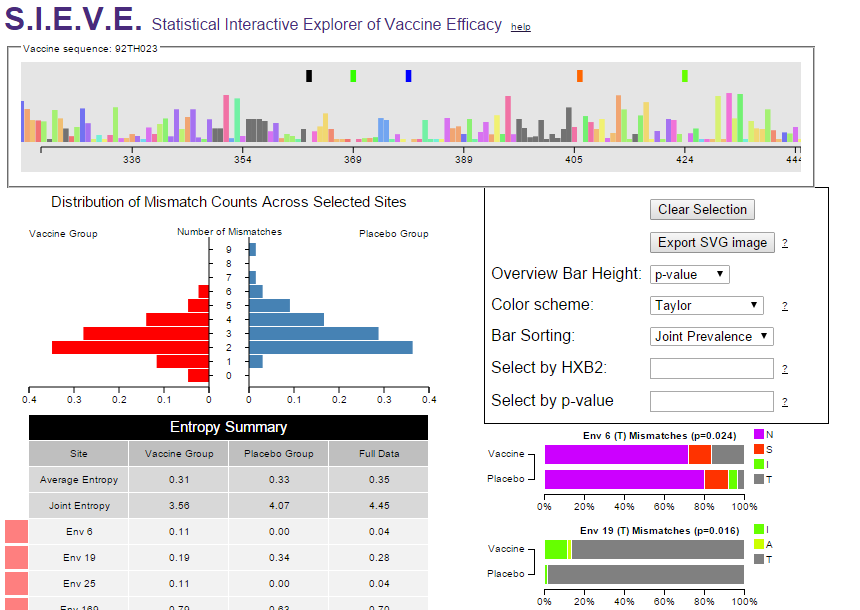
\includegraphics[height=3in,width=12in,clip=true,trim = 0in 6in 0 0]{overview.png}
\end{center}
\begin{itemize}
\item Each individual bar corresponds to a particular amino acid.
\item Bar height corresponds with a chosen measure of ''interestingness."
\item Zooming in/out facilitates navigation.
\end{itemize}

\subsubsection{Site-wise Comparisons}

\begin{itemize}
\item Stacked bar charts are a common visualization for displaying mutations from a reference sequence.
\item Different color schemes provide various aggregations of amino acids (based on chemical properties).
\item Charts are exportable as SVG files.
\end{itemize}

\subsubsection{Group Data}

\begin{itemize}
\item Pyramid plot provides a view of the distribution of mismatches for each group.
\item Table provides both aggregate and site-wise information as well as interactive elements for navigation.
\end{itemize}


\subsection{Tools}
We chose to accomplish this using the D3.js visualization library so that our web-based interface to be as accessible as possible to researchers in the field. In addition, planned features to aid in editing and exporting the graphic for inclusion in sieve analysis papers and we hoped to design it be easily extensible by researchers to add new features as they saw fit, such as different statistical measures and different data sets.


\section{Results}

\subsection{Final Product}

\begin{center}
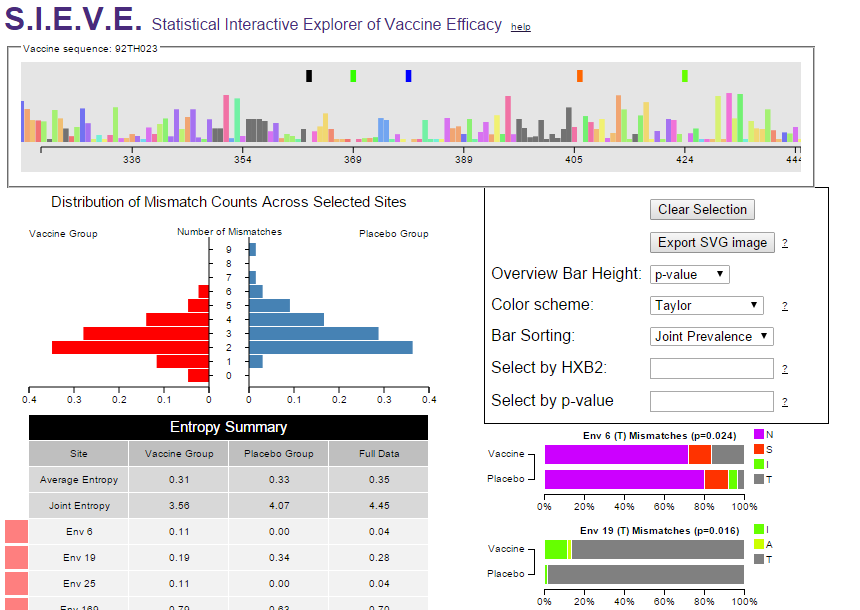
\includegraphics[height=9in,width=12in]{overview.png}
\end{center}
The positioning of the three main sections are based loosely on existing software with a site selection tool on the top of the page with summary and drilldown information available below.







\section{Future Work}
\begin{itemize}
\item Make the tool more broadly applicable and reduce restrictions on user input.
\item Add ability for researchers to share their findings.
\end{itemize}


\bibliographystyle{unsrt}
\bibliography{poster}{}


\end{poster}

\end{document}

 
